\subsection{Cerenkov Counter Cuts}
\subsubsection{ Osipenko (CC Geometry and Time Matching) Cuts}
\label{osiCuts}
As discussed in section \ref{cha:EG4}%{expSetUp} %Or refer directly to the CC section (by its own label, to be added)  (There were 18 modules in the old CC of of each CLAS sector)
the new EG4-dedicated CC consists of 11 modules %/segments 
each consisting of a pair %each 
of mirrors and PMTs. The segments are placed along the CLAS polar angle covering 15 to 45 degrees, i.e., the segments are at different polar angular positions. % See presentation cerenkov_son_july2003 (in the UbuntuOne/EG4nMore1/Jlab/Detector/CLASdetector/CC (also have a look at other presentations as well as E. Golovach's work on the Cerenkov (linked from EG4 wiki main page - http://www.ge.infn.it/~golovach/cerenkov/ (I can/may find a lot of plots and design diagrams))
During normal operation, the PMTs of these segments may produce %a certain amount of noise signal 
thermal noise that is equivalent to that produced by one photo-electron passing through it. As a result, when a noise pulse in the CC and a pion track measured by DC coincides within the trigger window of the CLAS detector, %Nevzat writes the window is 150 ns; thesis pg 145
the track gets registered as an electron candidate by the event reconstruction program, thus contributing to the contamination of electron candidates % samples 
with the misidentified pion tracks. In fact, this turns out to be the biggest source of pion contamination. In order to minimize such contamination and help better identify electrons from pions, %the 
CC geometric and time-matching cuts are applied.

%https://userweb.jlab.org/~ungaro/maureepage/proj/pi0/e_pid/note/electron_pid.html#x1-120001.9
%The cuts in this category
This category of cuts for this experiment is %by X. Zheng \cite{eg4wiki} - one of the collaborators of the experiment. Her work, in turn, was 
mostly based on a similar analysis done for another CLAS experiment by M. Osipenko \cite{cnOsipenko}.% in order to study the CC response and thereby develop a method to better discriminate electrons from pions. 


The first requirement in the CC-matching is for the electron candidate track (as reconstructed by DC) to have a corresponding signal in CC. In addition, the track needs to meet several %the following %GED
matching conditions to be acceptable as described in the next sections.


%\subsubsubsection{CC \th Matching} %http://tex.stackexchange.com/questions/186981/is-there-a-subsubsubsection-command
\paragraph{CC \th Matching}
As said above, the CC segments are at different average polar angle positions (between 15 and 45 degrees), so in principle, one can expect a one-to-one correspondence between the polar angle of the track (as measured at the vertex) and the CC-segment. However, the torus magnetic field bends the particles towards or away from the beamline, so it's more convenient to use the CC projected polar angle \thp  rather than the vertex angle $\theta$, where \thp is defined as the polar angle of the position vector defined by the point of intersection of the track with %the CC plane
the plane at which the CC PMTs reside as reflected by the CC mirrors %xz: I think instead of "the CC plane" you should say "the plane at which the CC PMTs reside as reflected by the CC mirrors."
(another projected angle \php is the azimuthal angle of the same vector). These projected angles can be uniquely calculated for each track based on the DC %and CC 
signals of the track as well as the CC geometry information. To simplify the later analysis process, these projected angles for each track were calcuated during the final %/pass1 version  of the
 data reconstruction process and then saved in the output files %(in ntuple-10 format)
  just like all the other %usual 
 information for the events and particles. 
Finally, for the actual electrons a one-to-one correspondence between \thp and the segment number can be established, 
which discriminates against %while the same cannot be done for the 
background noise and the accidental pions (or any other negative charge candidates). For each segment, the \thp distribution (see Fig. \ref{ccThProjDist}) is fitted with a gaussian %+ second order polynomial distribution
to determine its mean ($\mu$) and width ($\sigma$) and then saved for future use in cuts. These fit parameters are then used during the data analysis to define these CC-\th-matching cuts. The events that have $\mu-3\sigma<\theta_{proj}<\mu+3\sigma$ pass this cut, and the others are rejected as not genuinely being electrons. %\textbf{\textcolor{red}{Plots later ..}}
% http://wwwold.jlab.org/Hall-B//secure/eg4/adhikari/Analysis/SimStuffs/CutsPlots/eg4CutsNCorrections.html#osiCuts
%      if(fabs(theta-th_offset[isec-1][iseg-1]) < (3.0*th_wid[isec-1][iseg-1]))        	theta_p_cut= true;
%      else                                                                             theta_p_cut= false;
\begin{figure}[H] %[hp] %ht, htpb (p - float, b = bottom, h=? t = top)
\centering
%\leavevmode 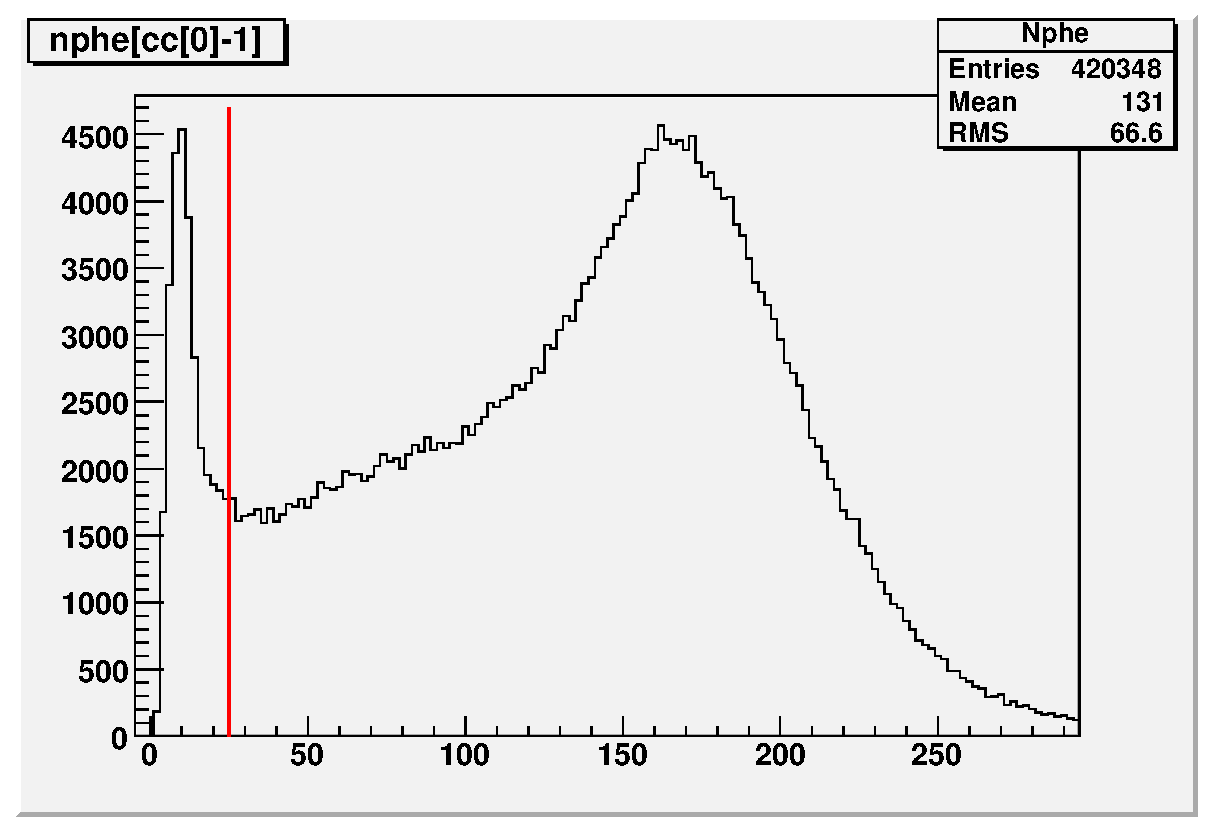
\includegraphics[width=0.8\textwidth]{TexmakerMyFinTh/chap4simul/FigCuts/npheCutFrmRtPrmtClasEb2.eps}  %0.6 is the fraction of the real image width????
\leavevmode 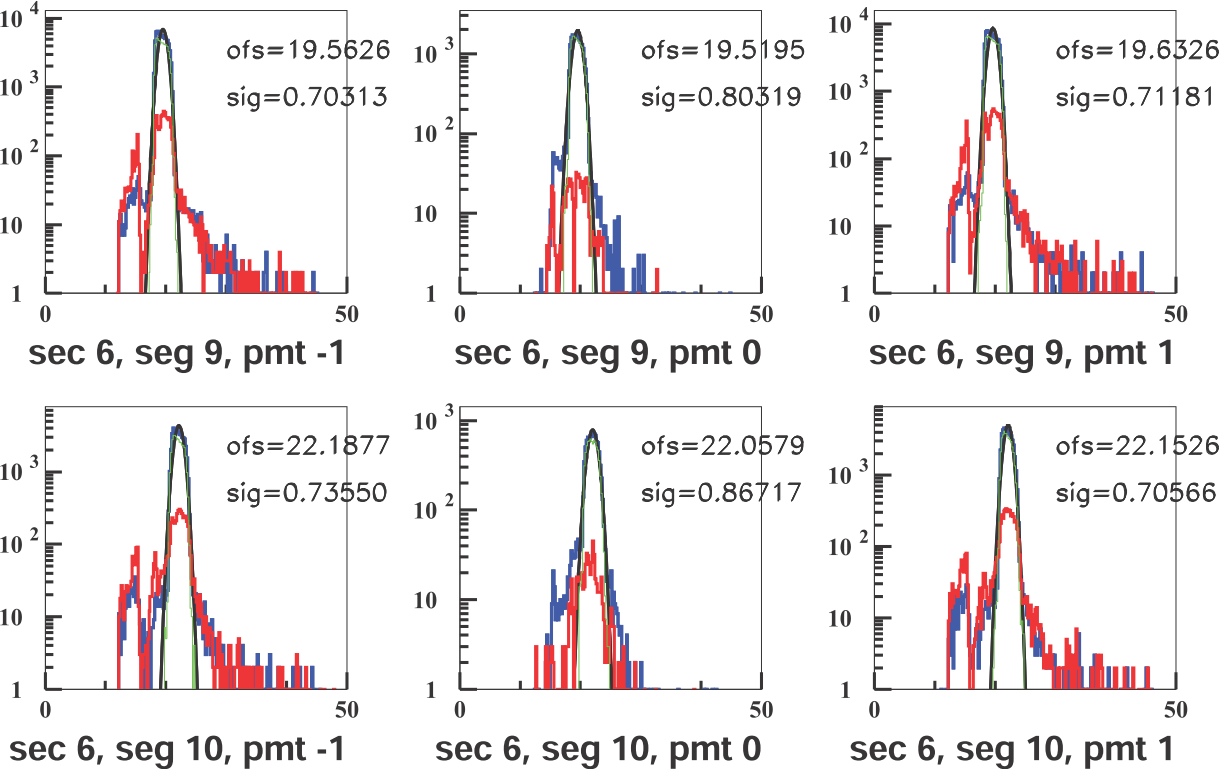
\includegraphics[width=1.0\textwidth]{TexmakerMyFinTh/chap4simul/FigCuts/ccOsipenkoXZhengNotePDFexportThProj}  %0.6 is the fraction of the real image width????
\caption[CC-projected \th distributions]{The \thp distributions %(from a carbon target run 50808) 
in two (9$^{th}$ and 10$^{th}$) of the CC-segments (figures used from \cite{anaNoteXZheng}). Here, the first, second and third columns correspond to events that fired the left, both and the right PMTs respectively. The \textcolor{blue}{blue} lines are for good electron candidates that pass the EC cuts as well as $Nphe > 2.5$. The \textcolor{red}{red} ones are for those that pass the EC cuts but with $Nphe < 2.5$ (thus likely pions), and the \textcolor{green}{green} are for those which pass both EC cuts and all Osipenko cuts. The Gaussian fits which are used to define the \th matching cuts are shown in \textcolor{black}{black} ("ofs" and "sig" in the panel refer to $\mu$ and $\sigma$, respectively). If the candidate falls outside $\pm 3 \sigma$ limits given by the fit, \thp is taken as not matching with the corresponding segment and, therefore, the event is rejected.}
\label{ccThProjDist}
\end{figure}
    

\paragraph{CC \ph Matching}
One can also have a one to one correspondence between the other CC-projected angle \php and the left or right PMT in the corresponding CC-segment, because when the track is on the right side of the CC, the right PMT should fire and vice versa. However, there are some exceptional cases of events which fire both PMTs. That happens when \php of the track is less than 4 degrees (when measured relative to the sector mid-plane), in which case the Cerenkov light hits both PMTs but with less efficiency %(because the energy is shared between the two).
(because the Cherenkov photons are shared between the two). Fig. \ref{ccPhProjDist} shows for two of the segments the \php distributions and the Gaussian fits that are used to define these cuts.
\begin{figure}[H] %[hp] %ht, htpb (p - float, b = bottom, h=? t = top)
\centering
%\leavevmode 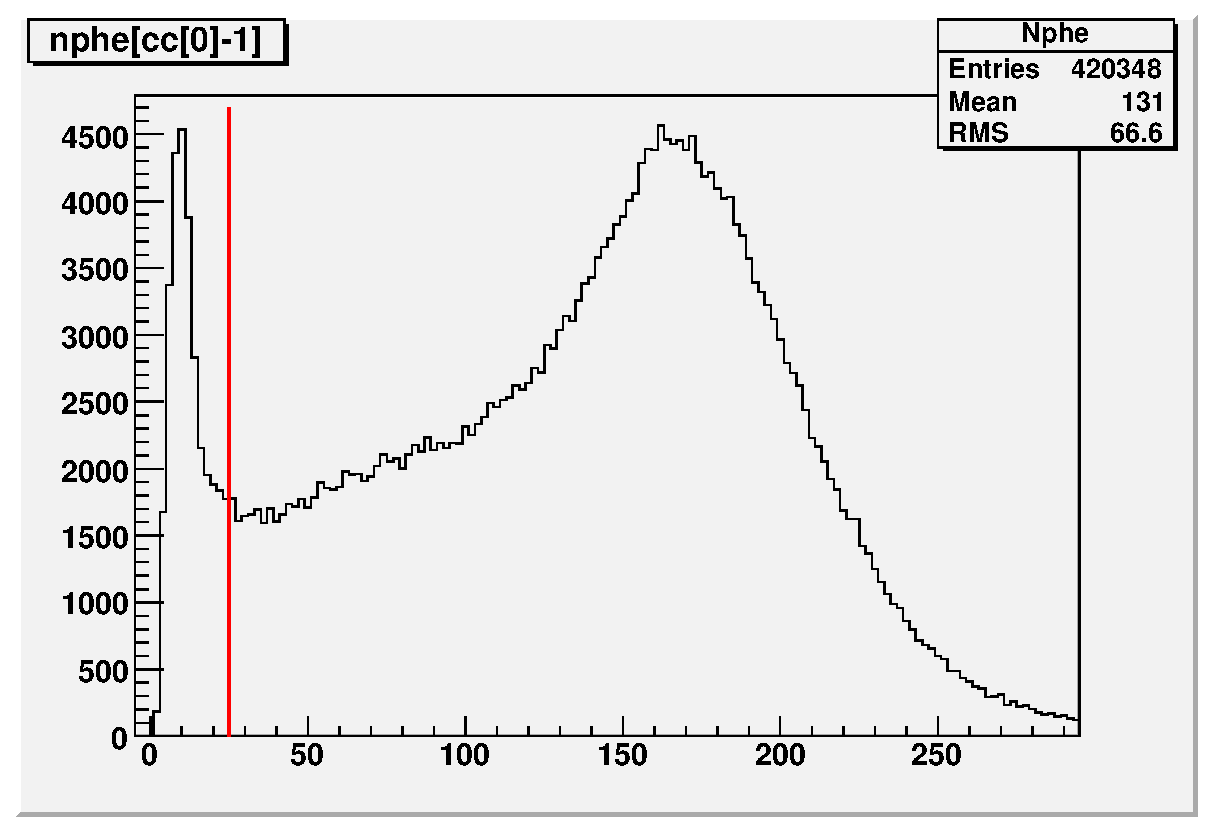
\includegraphics[width=0.8\textwidth]{TexmakerMyFinTh/chap4simul/FigCuts/npheCutFrmRtPrmtClasEb2.eps}  %0.6 is the fraction of the real image width????
\leavevmode 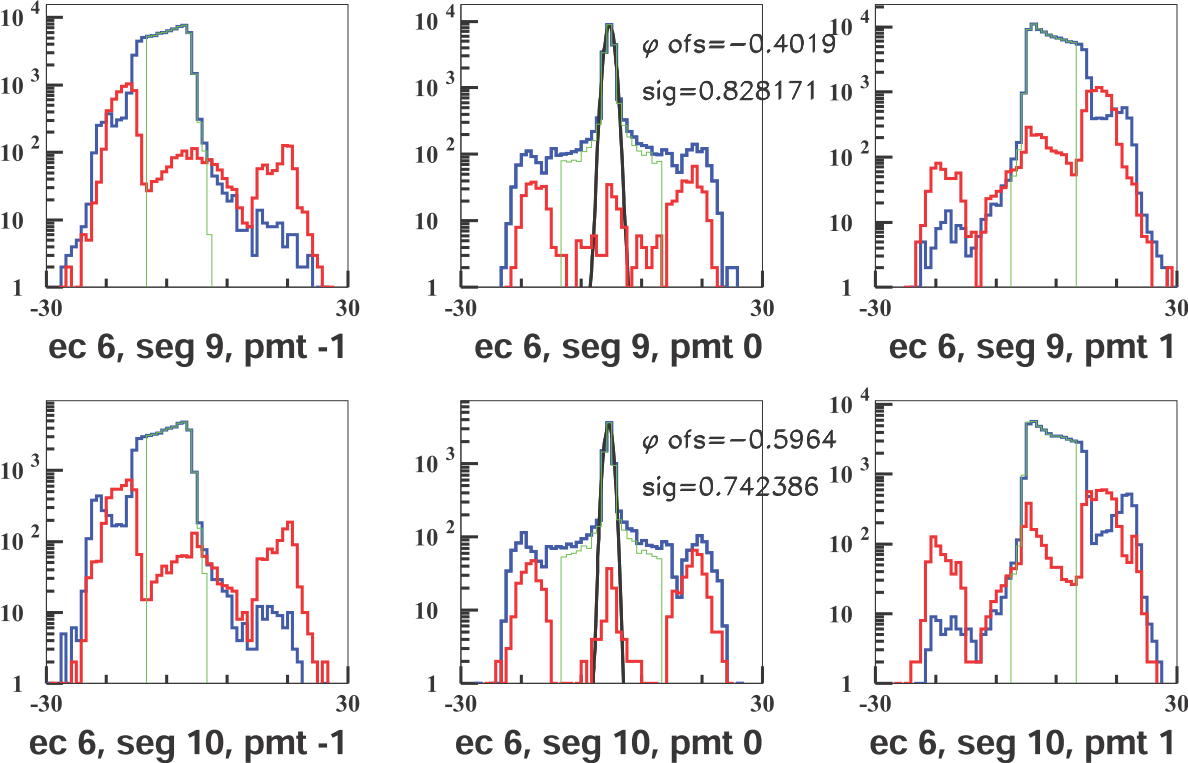
\includegraphics[width=1.0\textwidth]{TexmakerMyFinTh/chap4simul/FigCuts/ccOsipenkoXZhengNotePDFexportPhProj}  %0.6 is the fraction of the real image width????
\caption[CC-projected \ph distributions]{The \php distributions in two (9$^{th}$ and 10$^{th}$) of the CC-segments (figure used from \cite{anaNoteXZheng}). Here, the first, second and third columns correspond to events that fired the left, both and the right PMTs respectively. The \textcolor{blue}{blue} lines are for good electron candidates that pass the EC cuts as well as $Nphe > 2.5$. The \textcolor{red}{red} ones are for those that pass the EC cuts but with $Nphe < 2.5$ (thus likely pions), and the \textcolor{green}{green} are for those which pass both EC cuts and all Osipenko cuts. The Gaussian fits to the distributions that fired both left and right PMTs are shown in \textcolor{black}{black} ("ofs" and "sig" in the panel refer to $\mu$ and $\sigma$, respectively). If the candidate falls outside $3 \sigma$ on the positive (negative) side but the left (right) PMT is fired, we take it as having left-right inconsistency and, therefore, the event is rejected. In other words, if $\theta < \mu - 3 \sigma$ but $PMT=1$, or if $\theta > \mu + 3 \sigma$ but $PMT=-1$, the event is rejected.}
\label{ccPhProjDist}
\end{figure}

\paragraph{CC Time Matching}
The difference $\Delta T$ between the track time recorded on a CC segment and the corresponding time recorded on the TOF (or SC), corrected for the path length from the CC to the TOF, is used to define one of the time-matching cuts $\Delta t_{SC - CC} > - 6.0 ns$ which was chosen to reduce pion contamination without losing too many electron candidates (see Fig \ref{scCcTime}). Likewise, the time between CC and EC is also used to define another cut $\Delta t_{EC - CC} > - 6.0 ns$ (see Fig \ref{ecCcTime}) to further reduce the pion contamination.
% X. Zheng's wiki on the work: https://clasweb.jlab.org/rungroups/eg4/wiki/index.php/User:Xiaochao#Osipenko_cuts_study
%\textbf{\textcolor{red}{More details later ..}}

\begin{figure}[H] %[hp] %ht, htpb (p - float, b = bottom, h=? t = top)
\centering
\leavevmode 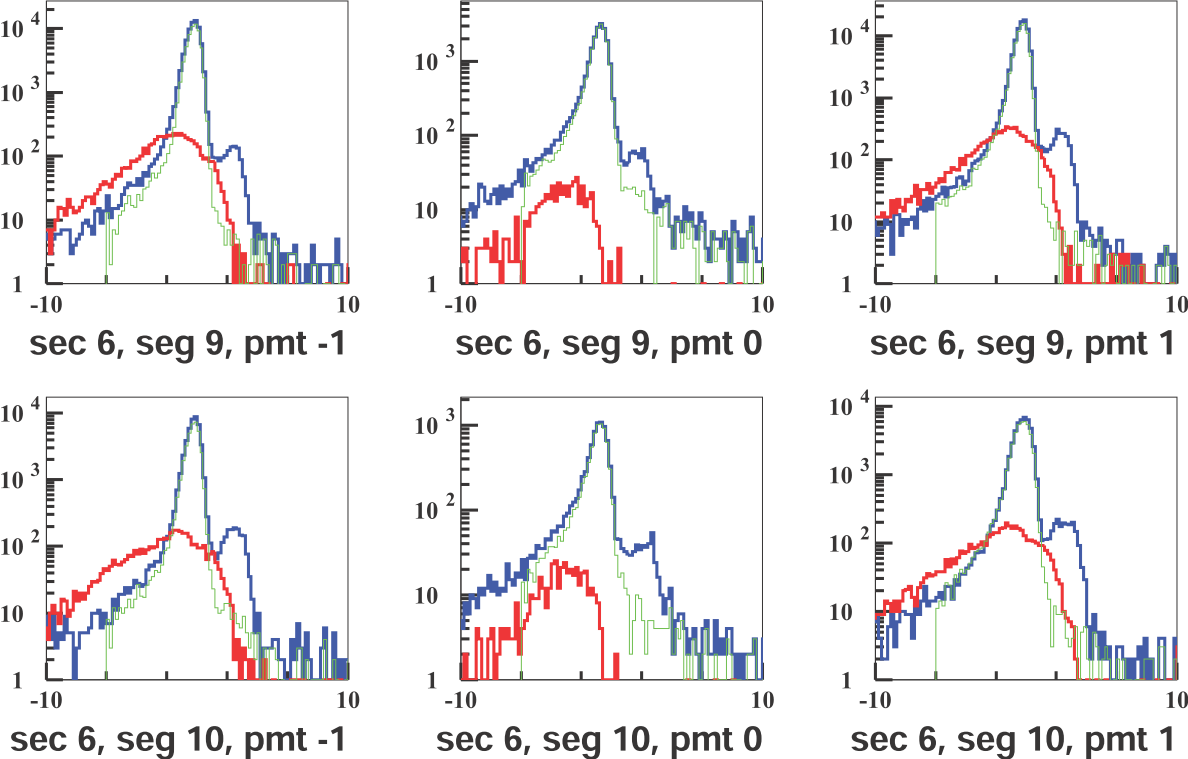
\includegraphics[width=1.0\textwidth]{TexmakerMyFinTh/chap4simul/FigCuts/ccOsipenkoXZhengNotePDFexportScCcTime}  
\caption[SC - CC Time]{The $\Delta t_{SC - CC}$ distributions for two of the CC-segments (figure used from \cite{anaNoteXZheng}). Here, the first, second and third columns correspond to events that fired the left, both and the right PMTs respectively. The \textcolor{blue}{blue} lines are for good electron candidates that pass the EC cuts as well as $Nphe > 2.5$. The \textcolor{red}{red} ones are for those that pass the EC cuts but with $Nphe < 2.5$ (thus likely pions), and the \textcolor{green}{green} are for those which pass both EC cuts and all Osipenko cuts. The $\Delta t_{SC - CC} > - 6.0 ns$ cut was chosen to reduce pion contamination without losing too many electron candidates. (The small peaks at about +3 ns are due to particles hitting PMTs directly.)}
\label{scCcTime}
\end{figure}

\begin{figure}[H] %[hp] %ht, htpb (p - float, b = bottom, h=? t = top)
\centering
\leavevmode 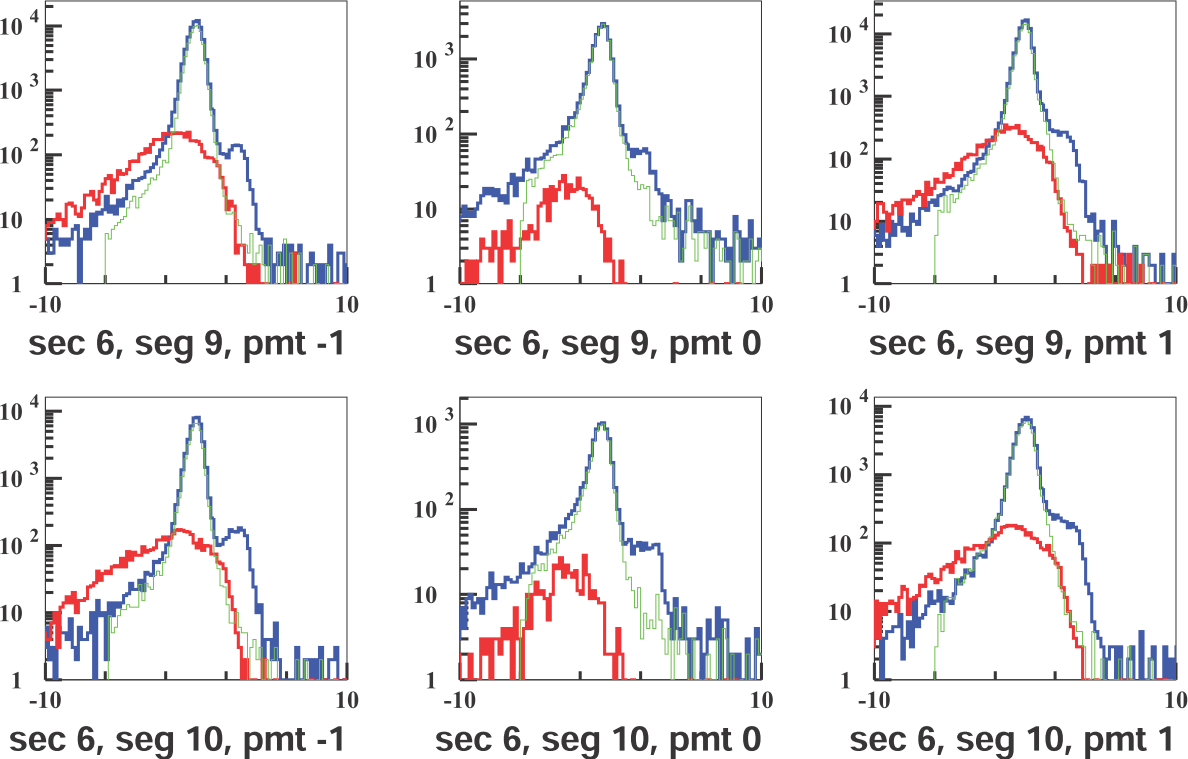
\includegraphics[width=1.0\textwidth]{TexmakerMyFinTh/chap4simul/FigCuts/ccOsipenkoXZhengNotePDFexportEcCcTime}  
\caption[EC - CC Time]{The $\Delta t_{EC - CC}$ distributions for two of the CC-segments (figure used from \cite{anaNoteXZheng}). Here, the first, second and third columns correspond to events that fired the left, both and the right PMTs respectively. The \textcolor{blue}{blue} lines are for good electron candidates that pass the EC cuts as well as $Nphe > 2.5$. The \textcolor{red}{red} ones are for those that pass the EC cuts but with $Nphe < 2.5$ (thus likely pions), and the \textcolor{green}{green} are for those which pass both EC cuts and all Osipenko cuts. The $\Delta t_{EC - CC} > - 6.0 ns$ cut was chosen to reduce pion contamination without losing too many electron candidates. (The small peaks at about +3 ns are due to particles hitting PMTs directly.)}
\label{ecCcTime}
\end{figure}




\subsubsection{Cut on Minumum Number of Photoelectrons}
\label{nphCut} 
%https://userweb.jlab.org/~ungaro/maureepage/proj/pi0/e_pid/note/electron_pid.html#x1-120001.9
The ``nphe'' variable in the data ntuple which represents the ADC signal from the CC converted to ``number of photoelectrons'' and multiplied by 10 is also used %one of the useful variables 
to discriminate electrons from pions and %electronic noise.
the background. %xz: what is this "electronic background"? First you have thermal noise, which in my opinion should really be just the general "background". Maybe should sjust say "background" here.
The number of photoelectrons produced in CC by an electron  is typically between 5 and 25 or between 50 and 250 in the units of nphe, where the electronic background and negative pions produce signals equivalent to one photo-electron (or 10 in nphe units) and so a cut is determined somewhere between these two regions based on the shapes and sizes of the electron and pion peaks. In our case, we chose to have the cut $Nphe > 25$ as depicted by the straight line in Fig. \ref{npheCt}.

\begin{figure}[] %[hp] %ht, htpb (p - float, b = bottom, h=? t = top)
\centering
%\leavevmode 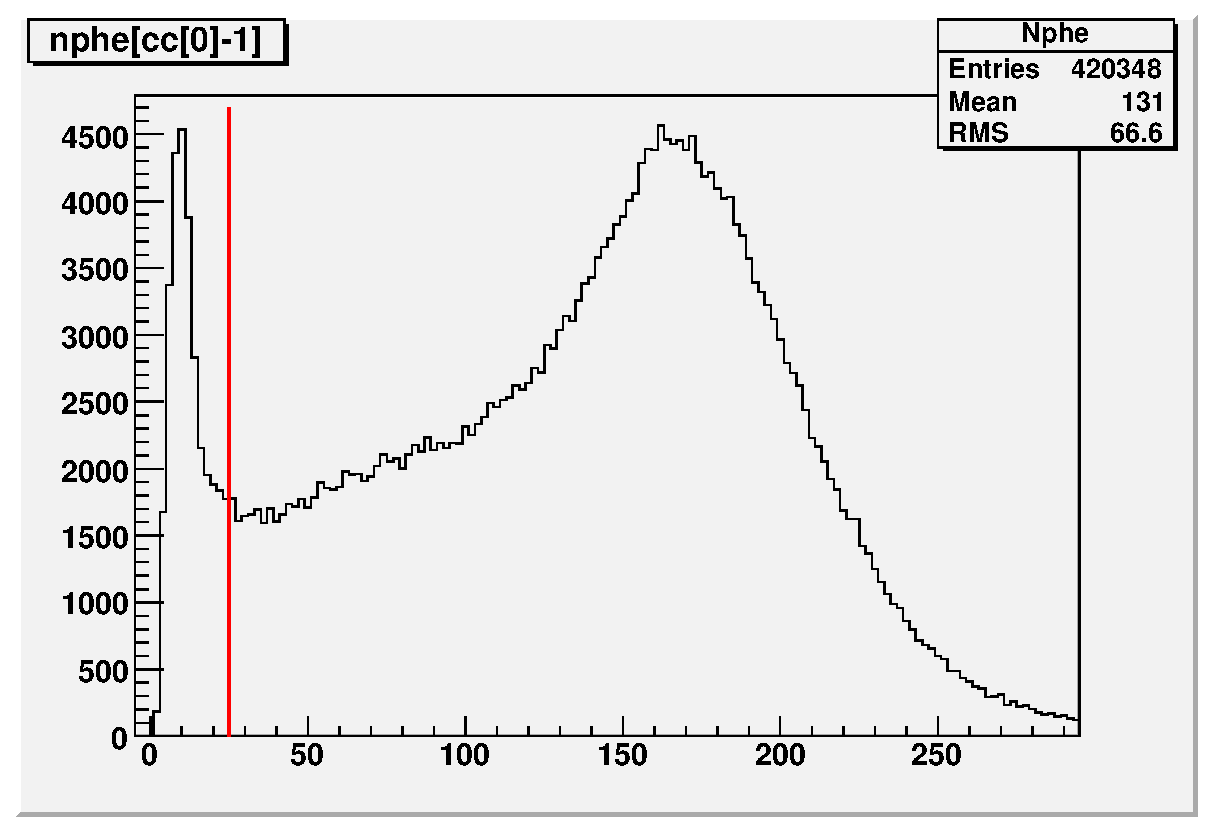
\includegraphics[width=0.8\textwidth]{TexmakerMyFinTh/chap4simul/FigCuts/npheCutFrmRtPrmtClasEb2.eps}  %0.6 is the fraction of the real image width????
\leavevmode 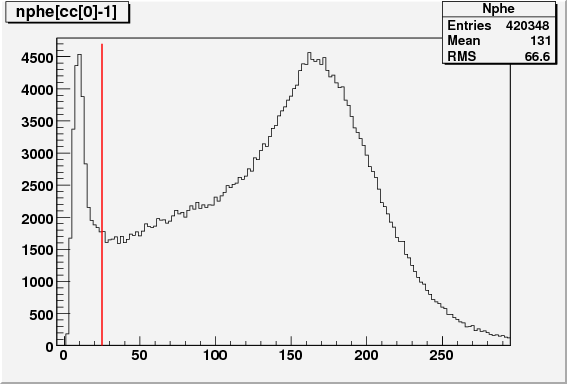
\includegraphics[width=0.6\textwidth]{TexmakerMyFinTh/chap4simul/FigCuts/npheCutFrmRtPrmtClasEb2}  %0.6 is the fraction of the real image width????
\caption[CC-photoelectron number cut]{The cut (the red straight line at 25) on the number of photo-electrons produced in CC times 10 (from 2.0 GeV data). The signals below the red line are mostly pions and noise and above the line are mostly electrons.
%\textcolor{red}{SEK: Show overlay with and without Osipenko cuts.}
}
\label{npheCt}
\end{figure}
